\chapter{\difficult{Quantization}}\label{chapter:quantization}

    The content of \namecrefs{chapter:principal_bundles}~\nameref{chapter:vector_bundles}, \nameref{chapter:principal_bundles} and~\nameref{chapter:symplectic} are prerequisites for the section on geometric quantization. References for the section on geometric quantization are~\citet{brylinski_loop_1993,tuynman_metaplectic_2016,bates_lectures_1997,camosso_prequantization_2021}. The section on Toeplitz quantization is mainly based on~\citet{hawkins_geometric_2000}. A general reference comparing deformation and geometric quantization is~\citet{hawkins_correspondence_1998}.

    \minitoc

\section{Introduction}

    Given the content of \cref{section:mathematical_formalism_qm}, the general quantization procedure for a dynamical system $(M,\omega,H)$ can be axiomatized as follows.
    \begin{method}[Abstract quantization]\label{quantization:axioms}\index{Dirac!correspondence}
        A quantization of a symplectic manifold $(M,\omega)$ is a pair $(\mathcal{H},\mathcal{O})$ where:
        \begin{itemize}
            \item $\mathcal{H}$ is a (complex) separable Hilbert space,
            \item $\mathcal{O}$ takes real functions $C^\infty(M)$ to self-adjoint operators,
            \item $\mathcal{O}$ is $\mathbb{C}$-linear,
            \item $\mathcal{O}(1) = \mathbbm{1}_{\mathcal{H}}$, and
            \item \textbf{Dirac correspondence}: $[\mathcal{O}(f),\mathcal{O}(g)] = i\hbar\mathcal{O}(\{f,g\}) + O(\hbar^2)$.
        \end{itemize}
    \end{method}
    \begin{remark}[$C^*$-bundles]\label{quantization:c_star_bundle_quantization}
        \Citet{hawkins_geometric_2000} defines a general quantization as a \textit{continuous bundle} $\pi:A\rightarrow[0,+\infty[$ \textit{of $C^*$-algebras} such that $\mathrm{ev}_0(\Gamma(A))=C^\infty(M)$. See \cref{section:toeplitz_quantization} for more information.
    \end{remark}

    Because a Hilbert space forms an irreducible representation of any complete set of observables, it makes sense to add an additional irreducibility axiom.
    \begin{axiom}[Irreducibility postulate]
        Let $(M,\omega)$ be a $2n$-dimensional symplectic manifold. If the observables $\{f_i\}_{i\leq n}$ form a complete set, i.e.~any function that Poisson commutes with all $f_i$ is necessarily constant, the quantum state space $\mathcal{H}$ is required to be irreducible with respect to the action of $\{\mathcal{O}(f_i)\}_{i\leq n}$. Equivalently, if a group $G$ acts transitively on $M$, the state space is required to be an irreducible representation of a $\mathrm{U}(1)$-central extension of $G$.
    \end{axiom}

    The simplest example is again $T^*\mathbb{R}^n$. Here, the usual choice of observables are the coordinate and momentum functions $\{q^i,p_i\}_{i\leq n}$ and the group $G$ is given by the \textit{Heisenberg group}, a $\mathrm{U}(1)$-central extension of the translation group $\mathbb{R}^{2n}$. Irreducible representations are characterized by the Stone--von Neumann theorem~\ref{qm_formalism:stone_von_neumann}.\index{Heisenberg!group}

    Although the above procedure sounds reasonable, it is known to be inconsistent. \textit{Groenewold} and \textit{Van Hove} showed that there does not exist a map $\mathcal{O}$, satisyfing the axioms~\ref{quantization:axioms}, that takes the entire (Lie) algebra of classical observables to the (Lie) algebra of corresponding quantum observables. As such, a different approach should be followed.\index{Groenewold--Van Hove}

\section{Deformation quantization}\index{quantization|seealso{deformation}}

    \newdef{Formal deformation quantization}{\index{star product}
        Let $A$ be a Poisson algebra. A \textbf{star product} on $A$ is an associative, $\mathbb{R}$-bilinear product on $A[[\hbar]]$ such that for all $a,b\in A$:
        \begin{gather}
            a\ast b = \sum_{i=0}^{+\infty}B_i(a,b)\hbar^i
        \end{gather}
        with $B_0(a,b) = ab$. A formal deformation quantization of $A$ is a star product such that
        \begin{gather}
            \{a,b\} = B_1(a,b) - B_1(b,a)\,.
        \end{gather}
    }

    \newdef{Moyal deformation quantization}{\index{deformation quantization!Moyal}\index{Poisson!vector space}\index{manifold!linear Poisson}\label{quantization:moyal}
        Let $V$ be a Poisson vector space\footnote{Also called a \textbf{linear Poisson manifold}.}, i.e.~a vector space equipped with a Poisson bivector $\pi\in V\wedge V$. The ring $C^\infty(V)[[\hbar]]$ can be equipped with the following product:
        \begin{gather}
            f\ast g := \mu\circ\exp(\hbar\pi)(f\otimes g)\,,
        \end{gather}
        where $\pi$ is viewed as an endomorphism on $C^\infty(V)\otimes C^\infty(V)$ and $\mu$ is the ordinary product map.
    }

    \newdef{Fedosov deformation quantization}{\index{deformation quantization!Fedosov}
        Consider a symplectic manifold $(M,\omega)$. Every tangent space $T_pM$ carries the structure of a Poisson vector space and, hence, admits a Moyal quantization $(T_pM,\ast_\omega)$. These spaces can be turned into an algebra bundle $\mathcal{A}$ over $M$. It can, moreover, be shown that any such bundle admits at least one flat connection that respects the algebra structure and such that there exists an isomorphism as follows:
        \begin{gather}
            \ker(\nabla^{\text{Fed}})\cong C^\infty(M)[[\hbar]]\,.
        \end{gather}
        This connection is called a \textbf{Fedosov connection}. The restriction of the star product on $\Gamma(\mathcal{A})$ to this subbundle gives a formal deformation quantization of $C^\infty(M)$.
    }
    \begin{remark}[Kontsevich quantization]\index{Kontsevich quantization}
        \textit{Kontsevich} had previously proven that every finite-dimensional Poisson manifold admits a deformation quantization of its algebra of smooth functions. However, a slight variation of Fedosov's approach can be used even for infinite-dimensional algebras such as those occuring in field theory (where Kontsevich's approach is invalid).
    \end{remark}

\section{Geometric Quantization}\label{section:geometric_quantization}

    In this section, the natural constant $\hbar$ has been set to 1.

\subsection{Prequantization}

    \newdef{Prequantum line bundle}{\index{pre-!quantum line bundle}
        Consider a symplectic manifold $(M,\omega)$. A prequantum line bundle on $M$ is a Hermitian line bundle equipped with a connection $\nabla$ such that $\omega=F_\nabla$, where $F_\nabla$ denotes the curvature of $\nabla$.
    }
    \begin{property}\index{Weil!integrality}\index{Dirac!condition}\index{Bohr--Sommerfeld condition}
        Complex line bundles are classified by the (first) Chern class $c_1\in H^2(M;\mathbb{Z})$, which is proportional to the curvature form through Chern--Weil theory. Therefore, a prequantum line bundle exists if and only if the symplectic form is integral (up to a factor of $2\pi$). For simply connected manifolds, this is equivalent to
        \begin{gather}
            \forall S\in H_2(M):\Int_S\omega\in 2\pi\mathbb{Z}\,.
        \end{gather}
        This condition resembles the `old' \textit{Bohr--Sommerfeld condition}\footnote{In fact, it is closer to Einstein's quantization rule~\citep{stone_einsteins_2005}.} and is, in general, known as the \textbf{Weil integrality condition}.

        There are two contributions to the moduli space of prequantum line bundles or, essentially, $\mathrm{U}(1)$-principal bundles with connection. The latter are known to be classified by differential $\mathrm{U}(1)$-cohomology as shown in \cref{section:differential_cohomology}. Since the curvature is fixed by the sympletic form, prequantum line bundles are classified by lifts from curvature forms to differential cohomology along the curvature projection. Differential cohomology consists of two parts, roughly corresponding to the following two aspects: there can exist topologically inequivalent bundles and there can exist inequivalent connections on the same bundle differing by a flat connection, where two flat connections are in turn inequivalent if they differ by a closed one-form that is neither integral nor exact. The former are classified by integral curvature forms $H^2_{\text{dR}}(M)$, while the latter are classified by the \v{C}ech cohomology group $H^1(M;\mathrm{U}(1))$ or, equivalently by isomorphism~\eqref{bundle:U1_cohomology_isomorphism}, $H^2(M;\mathbb{Z})$.
    \end{property}
    \begin{result}[Dirac quantization condition]
        One can derive the Dirac quantization condition from Weil integrality. If one couples the system to a gauge potential, the minimal coupling procedure gives $\omega\longrightarrow\omega+eF$. Weil integrality then implies that $e$ is an integer.
    \end{result}

    \newdef{Prequantum Hilbert space}{\index{Segal--Kostant--Souriau procedure}
        Consider a symplectic manifold $(M,\omega)$ together with a prequantum line bundle $L$. The prequantum Hilbert space $\mathcal{H}_L$ is defined as (the $L^2$-completion of) the space of square-integrable sections of $L$ with respect to the metric on $L$ and the Liouville volume form on $M$.

        To every smooth function $f\in C^\infty(M,\mathbb{C})$, one can associate a (\textbf{Segal--Kostant--Souriau}) prequantum operator $\widehat{f}:\Gamma(L)\rightarrow\Gamma(L)$ by the following formula:
        \begin{gather}
            \widehat{f}:\psi\mapsto f\cdot\psi-i\nabla_{X_f}\,\psi\,,
        \end{gather}
        where $X_f$ is the Hamiltonian vector field associated to $f$ and, locally,
        \begin{gather}
            \nabla = \dr - i\theta
        \end{gather}
        with $\theta$ the symplectic potential. This operator can also be interpreted in terms of a Hamiltonian flow. The Hamiltonian flow of $X_f$ can be lifted (up to a phase) to an automorphism $\psi_t[f]$ on $L$ that preserves both the metric and the connection. The prequantum operator $\widehat{f}$ is then simply given by
        \begin{gather}
            \widehat{f}s = -i\left.\deriv{}{t}(\psi_t[f]s)\right|_{t=0}\,.
        \end{gather}
    }

    \begin{example}[Spinning particle]\index{spin}
        Consider as phase space the 2-sphere $S^2(r)$ with radius $r\in\mathbb{R}$. In this case, the symplectic form can be written as $\omega=r^2\sin\theta\dr\theta\wedge\dr\varphi$. This form is only integral for a discrete set of values of $r$, namely for $r\in\mathbb{Z}/2$. Up to a factor $\hbar$, this is exactly the quantization rule for the angular momentum. The reason is that $S^2$ is a homogeneous space for $\mathrm{SU}(2)$, the group characterizing spinning particles. In fact, using the theory of coadjoint orbits (see further below), one can show that this quantization procedure coincides with the \textit{KKS quantization} of the coadjoint orbit $S^2=\mathrm{SU}(2)/\mathrm{U}(1)$.
    \end{example}

    At this point, it can easily be seen that there is a problem with the dimension of the prequantum state space. For the cotangent bundle $T^*\mathbb{R}^n\cong\mathbb{R}^n\times\mathbb{R}^n$, the resulting state space would be $L^2(\mathbb{R}^{2n},\mathbb{C})$. However, from ordinary quantum theory it is well-known that the right Hilbert space is $L^2(\mathbb{R}^n,\mathbb{C})$. In general, the above procedure would give wave functions that depend on $2n$ variables instead of the $n$ coordinates of configuration space that are normally found in quantum mechanics. A solution is obtained by making a choice of `configuration space' or, in terms of ordinary quantum mechanics, to choose a `representation' of the system.
    \begin{construct}[Geometric quantization]\index{quantization!geometric}\index{polarization}
        Let $(M,\omega)$ be a symplectic manifold. A (geometric) quantization of $(M,\omega)$ is given by a prequantum line bundle $L$ together with a polarization $\mathcal{P}$ of $M$. The `naive' modification of the quantum state space is given by the subspace of $\mathcal{H}_L$ of those sections that are covariantly constant along $\mathcal{P}$, i.e.~those sections $s\in\Gamma(L)$ that satisfy $\nabla_Xs=0$ for all $X\in\mathcal{P}$. These sections are also called \textbf{polarized sections}.

        The fact that a polarization is required, and not merely an $n$-dimensional involutive distribution, follows from an additional consistency condition imposed by the condition $\nabla_Xs=0$ for all $X\in\mathcal{P}$. Because $\omega$ also represents the curvature of the connection on $L$, one obtains
        \begin{gather}
            \omega(X,Y)s = [\nabla_X,\nabla_Y]s - \nabla_{[X,Y]}s = 0
        \end{gather}
        for all $X,Y\in\mathcal{P}$. This implies that $\mathcal{P}$ defines an isotropic submanifold. For a completely integrable system, a natural choice would be given by the distribution spanned by the Hamiltonian vector fields.

        Now, if the prequantum operators ought to represent genuine operators on the quantum state space, one should have
        \begin{gather}
            \nabla_Xs=0\implies\nabla_X(\widehat{f}s)=0
        \end{gather}
        for all sections $s\in\Gamma(L)$ and $X\in\mathcal{P}$. Using the general formula for iterated covariant derivatives and the fact that the leaves of $P$ are Lagrangian, one finds the following condition:
        \begin{gather}
            [X,X_f]=0
        \end{gather}
        for all $X\in\mathcal{P}$. So, in general, one should restrict to the subspace of $C^\infty(M)$ on those functions whose Hamiltonian flow preserves $\mathcal{P}$.

        There is, however, a problem with this construction. Nothing ensures that $\mathcal{H}_L$ contains any polarized sections. As an example, consider a cotangent bundle with its vertical polarization. In this case, the polarized sections are given by functions that only depend on the base coordinates $q^i$ and not on the fibre (momentum) coordinates $p_i$. However, because the fibres are noncompact, the integral of such a section with respect to the Liouville measure will always diverge. This particular issue can be resolved by integrating over the leaf space $M\cong T^*M/D$, where $D$ is the isotropic foliation associated to $\mathcal{P}$.
    \end{construct}

    However, even though a possible divergence coming from noncompact fibres is resolved, another problem arises. To be able to integrate over a manifold one needs a volume form, but there is not always a canonical choice available. A solution is given by working with densities.
    \begin{method}[Half-form quantization]\index{quantization!half-form}\index{metaplectic!correction}\label{quantization:half_form}
        For this method, the polarization is assumed to be real and have simply connected leaves. Furthermore, the manifold $M$ is assumed to admit a metaplectic structure or, by virtue of \cref{complex:metaplectic}, $\mathcal{P}$ is assumed to admit a metalinear structure. (A choice of such a metaplectic structure is called a \textbf{metaplectic correction}.) Using this structure, one can define the half-form bundle $\delta^{1/2}$. Given a prequantum line bundle $L$, one defines the twisted bundle of $L$-valued half-forms $L\otimes\delta^{1/2}$. A \textbf{wave function} is defined as a section $\psi\in\Gamma(L\otimes\delta^{1/2})$ such that, locally, $\psi=\lambda\otimes\mu$ with $\nabla_X\lambda=0$ and $\mathcal{L}_X\mu=0$ for all $X\in\overline{\mathcal{P}}$. By pairing two wave functions, one obtains a 1-density on $M$ that can be integrated. The quantum state space is then defined as the $L^2$-completion of the space of wave functions.

        To extend the definition of operators to half-form quantized manifolds, one simply needs to extend the definition to density bundles. Because $\widehat{f}$ represents the Hamiltonian flow, a natural choice is the Lie derivative:
        \begin{gather}
            \widehat{f}(s\otimes\mu) := (\widehat{f}s)\otimes\mu - is\otimes\mathcal{L}_{X_f}\mu\,.
        \end{gather}
    \end{method}

    \begin{example}[K\"ahler quantization]\index{Segal--Bargmann representation}\index{Bargmann|see{Segal--Bargmann}}\index{quantization!K\"ahler}
        For this method, the polarization is assumed to be positive K\"ahler, i.e.~$P$ is the antiholomorphic tangent bundle of a K\"ahler manifold. By taking the (local) symplectic potential to be the holomorphic derivative of the K\"ahler potential, one obtains the space of holomorphic sections as the prequantum state space (a different choice of potential results in a phase transformation). It can be shown that a natural inner product is given by
        \begin{gather}
            \langle\psi_1\mid\psi_2\rangle = \Int_{\mathbb{C}^n}\overline{\psi_1}(z)\psi_2(z)\exp(-|z|^2/2)\,dz^n\,.
        \end{gather}
        This is often called the \textbf{Bargmann}, \textbf{Segal--Bargmann} or \textbf{Bargmann--Fock} representation. The coordinates $z,\overline{z}$ are represented by the operators $z$ and $\partial_z$. These correspond to creation and annihilation operators.
    \end{example}
    \begin{remark}
        If the positivity assumption would be dropped, the K\"ahler potential $K$, which was $-|z|^2/2$ above, would be indefinite. This would, in turn, imply that the integral diverges.
    \end{remark}
    \begin{remark}
        Recall \cref{section:kahler_dirac_operator}. If $M$ is compact K\"ahler, the existence of a metaplectic correction is equivalent to the existence of a spin structure. This leads to the $L$-twisted Dolbeault--Dirac operator:
        \begin{gather}
            \overline{\partial}_\nabla+\overline{\partial}\vphantom{\partial}_\nabla^\dagger:\Omega^{0,\bullet}(M)\otimes L\otimes\delta^{1/2}\rightarrow\Omega^{0,\bullet}(M)\otimes L\otimes\delta^{1/2}\,.
        \end{gather}
        From the perspective of the Dolbeault complex, the differential is twisted by a metaplectically corrected prequantum line bundle, but from the perspective of the Dirac operator, one only twists by the line bundle.
    \end{remark}

    \begin{method}[Bohr--Sommerfeld quantization]\index{Bohr--Sommerfeld condition}\index{Bohr--Sommerfeld variety}
        Here, the polarization $\mathcal{P}$ is again assumed to be real, but the leaves are not required to be simply connected. The connection $\nabla$ along $\mathcal{P}$ is flat when restricted to a single leaf $\Lambda_m\subset M$. When $\Lambda_m$ is not simply connected, the holonomy group can be nontrivial. However, the defining condition of $\mathcal{H}$ is that sections should be covariantly constant. This implies that either the section is zero or that the holonomy around any loop vanishes. The support of all sections in $\mathcal{H}$ is, therefore, given by the union $S$ of all leaves on which $\nabla$ is trivial. This space is called the \textbf{Bohr--Sommerfeld variety}.

        Vanishing holonomy implies
        \begin{gather}
            \exp\left(i\Oint_\gamma\theta\right) = 1
        \end{gather}
        for all loops $\gamma$, where $\theta$ is the symplectic potential. In terms of Darboux coordinates, this gives (up to a factor $2\pi$)
        \begin{gather}
            \Oint_\gamma p_i\,\dr q^i\in\mathbb{Z}\,.
        \end{gather}
        This is exactly the old Bohr--Sommerfeld quantization condition. When using half-density quantization, an additional contribution coming from the covariant derivative on densities would have to be added to the right-hand side:
        \begin{gather}
            \Oint_\gamma p_i\,\dr q^i = 2\pi(k_\gamma + d_\gamma)\,,
        \end{gather}
        where $k_\gamma\in\mathbb{Z}$.
    \end{method}

    \newdef{Bohr--Sommerfeld leaf}{\index{Bohr--Sommerfeld leaf}
        More generally, a Lagrangian submanifold $L$ of a prequantized symplectic manifold $(M,\omega)$ is said to be a \textbf{Bohr--Sommerfeld leaf} if $[\nabla_L]$ vanishes in $H^2_{\text{conn}}(L)$, the differential cohomology of $L$ (\cref{section:differential_cohomology}). On simply connected manifolds, this is equivalent to having trivial holonomy.

        This can be restated in terms of lifts to differential cohomology. The prequantization of a symplectic manifold is a lift as shown in the following diagram:
        \begin{gather}
            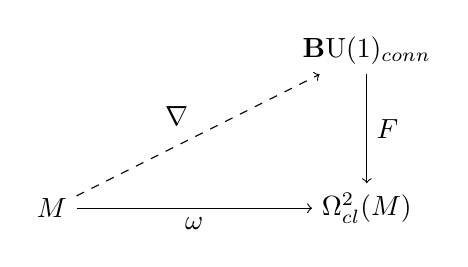
\begin{tikzpicture}[baseline = (current bounding box.center)]
                \node (M) at (0, 0) {$M$};
                \node (cl) at (4, 0) {$\Omega^2_{\text{cl}}(M)$};
                \node (H) at (4, 2) {$\mathbf{B}\mathrm{U}(1)_{\text{conn}}$};
                \draw[->] (M) -- node[below]{$\omega$} (cl);
                \draw[->] (H) -- node[right]{$F$} (cl);
                \draw[->, dashed] (M) -- node[above left]{$\nabla$} (H);
            \end{tikzpicture}
        \end{gather}
        where $\mathbf{B}\mathrm{U}(1)_{\text{conn}}$ is the Deligne complex (\cref{bundle:deligne_complex}). A submanifold $L\subset M$ is isotropic (Lagrangian if it is maximal) if the lift
        \begin{gather}
            \begin{tikzpicture}[baseline = (current bounding box.center)]
                \node (L) at (-2, 0) {$L$};
                \node (M) at (0, 0) {$M$};
                \node (cl) at (4, 0) {$\Omega^2_{\text{cl}}(M)$};
                \node (H) at (4, 2) {$\mathbf{B}\mathrm{U}(1)_{\text{conn}}$};
                \draw[right hook->] (L) -- (M);
                \draw[->] (M) -- node[below]{$\omega$} (cl);
                \draw[->] (H) -- node[right]{$F$} (cl);
                \draw[->, dashed] (M) -- node[above left]{$\nabla$} (H);
            \end{tikzpicture}
        \end{gather}
        is trivial in $H^2_{\text{conn}}(L)$.
    }

\subsection{Coadjoint orbits}

    \todo{COMPLETE (SEE ALSO \cref{section:coadjoint_orbits})}

\section{Toeplitz quantization}\label{section:toeplitz_quantization}

    \newdef{$C^*$-algebra bundle}{\index{C$^*$-algebra!bundle}\label{quantization:c_algebra_bundle}
        A (continuous) bundle of $C^*$-algebras over a locally compact Hausdorff space $X$ is a bundle $\pi:A\rightarrow X$ such that:
        \begin{enumerate}
            \item $\pi^{-1}(x)$ is a $C^*$-algebra for all $x\in X$.
            \item $\Gamma(A)$ is a $C^*$-algebra.
            \item $\mathrm{ev}_x(\Gamma(A))$ is dense in $\pi^{-1}(x)$ for all $x\in X$.
            \item $\mathrm{ev}_x$ is a $\ast$-epimorphism for all $x\in X$.
            \item For all $\nu\in\Gamma(A)$,
                \begin{gather}
                    \|\nu\| = \sup_{x\in X}\|\nu(x)\|\,.
                \end{gather}
            \item For all $f\in C_0(X)$ and $\nu\in\Gamma(A)$, there exists a $\nu_f\in\Gamma(A)$ such that $\nu_f(x)=f(x)\nu(x)$ for all $x\in X$.
            \item\textbf{Continuity}: For all $\nu\in\Gamma(A)$, the map $x\mapsto\|\nu(x)\|$ is in $C_0(X)$.
        \end{enumerate}

        \todo{CHECK DEFINITION (difference between field and bundle of algebras)}
    }

    In the remainder of this section, $M$ will be assumed to be a compact, connected K\"ahler manifold. Moreover, consider a prequantization $L$ and a Hermitian line bundle $L_0$. For all $n\in\mathbb{N}$, consider the line bundle $L\otimes L_0^n$, assumed to be positive (\cref{complex:positive_bundle}) with its Hilbert space of holomorphic sections $\mathcal{H}_n$ (which is finite dimensional by \cref{complex:holomorphic_sections}).

    \newdef{Toeplitz quantization}{\index{Toeplitz!quantization}\index{Toeplitz!operator}\index{Hardy space}
        The map $\mathfrak{T}_n:C^\infty(M)\rightarrow\mathrm{End}(\mathcal{H}_n)$ given by\footnote{This particular form, first multiplying by a smooth function and then projecting onto holomorphic sections, is very similar to the definition of \textit{Toeplitz operators}, where the projection is onto the \textit{Hardy space}, hence the name.}
        \begin{gather}
            \mathfrak{T}_n(f) := \pi_n\circ f\,,
        \end{gather}
        where $\pi_n:\Gamma(L\otimes L_0)\rightarrow\mathcal{H}_n$ is the canonical projection onto holomorphic sections. It can be shown that $\mathfrak{T}_n$ is unital and completely positive.

        To generalize this procedure to vector bundles, note that the Kodaira vanishing theorem (\cref{complex:kodaira_vanishing}) implies that the kernel of the $L\otimes L_0^n$-twisted Dolbeault operator $\overline{\partial}$ is concentrated in degree 0 and, hence, that
        \begin{gather}
            \ker(\overline{\partial}) = \mathcal{H}_n\,.
        \end{gather}
        The appropriate generalization to vector bundles will be the $E^*\otimes L\otimes L_0^n$-twisted Dolbeault--Dirac operator $D_E$ from \cref{complex:dolbeault_dirac_operator}:
        \begin{gather}
            \mathfrak{T}_n:\Gamma(E)\rightarrow\hom\bigl(\ker(D_E),\mathcal{H}_n\bigr):\sigma\mapsto\pi_n\circ\sigma\,,
        \end{gather}
        where multiplication by $\sigma$ is defined through the natural pairing of $E$ and $E^*$.

        Now, the Toeplitz maps $\mathfrak{T}_n$ piece together to give an operator $\mathfrak{T}:C^\infty(M)\rightarrow\prod_{n\in\mathbb{N}}\End(\mathcal{H}_n)$. This operator induces an isomorphism
        \begin{gather}
            \mathcal{T}:C^\infty(M)\cong \mathbb{A}/\mathbb{A}_0\,,
        \end{gather}
        where $\mathbb{A}_0:=\bigoplus_{n\in\mathbb{N}}\End(\mathcal{H}_n)$ and $\mathbb{A}:=\mathbb{A}_0\oplus\im(\mathfrak{T})$.

        A general quantization, in the sense of \cref{quantization:c_star_bundle_quantization}, is now given by the fact that there exists a bundle $A\rightarrow\widehat{\mathbb{N}}$, with $\widehat{\mathbb{N}}$ the one-point compactification$ \{0,\ldots,+\infty\}$, such that $\Gamma(A)=\mathbb{A}$, $A_n=\End(\mathcal{H}_n)$ for all $n\in\mathbb{N}$, and $A_{+\infty} = \mathcal{T}^{-1}\circ\pi_{\mathbb{A}_0}(\mathbb{A})$. 
    }

    \begin{remark}
        An equivalent quantization can be obtained from the operators
        \begin{gather}
            \mathfrak{Q}_n(f) := \mathfrak{T}_n\left(f + \frac{\Delta f}{2n}\right)\,.
        \end{gather}
    \end{remark}

    \todo{COMPLETE (\citet{hawkins_geometric_2000})}

\section{Constrained systems}\label{section:quantum_constrained}

    In this section, classical systems with constraints, i.e.~dynamical systems $(M,\omega,H)$ with an algebra of first-class constraints $\{\phi_a\}_{a\in I}$, are considered as in \cref{chapter:constrained_dynamics}.

\subsection{Dirac procedure}

    The first approach to the quantization of constrained systems is due to \textit{Dirac}. Instead of trying to pass to the reduced phase space or introducing additional gauge fixing conditions, \textit{Dirac} simply worked with all variables and represented these as operators acting on an enlarged Hilbert space. The constraints, represented by operators $\widehat{G}_a$, satisfy
    \begin{gather}
        \widehat{G}_a\ket{\psi}=0
    \end{gather}
    for all physical states $\ket{\psi}$. The constraint algebra $\{\phi_a,\phi_b\} = C^c_{ab}\phi_c$ gives rise to a quantum algebra
    \begin{gather}
        [\widehat{G}_a,\widehat{G}_b] = i\hbar\,C^c_{ab}\widehat{G}_c + \hbar^2\widehat{D}_{ab}\,,
    \end{gather}
    where $\widehat{D}_{ab}$ represents a \textbf{quantum anomaly}\index{anomaly}, i.e.~a correction term resulting from the quantization of the classical algebra (e.g.~operator ordering). The issue here is that both the left-hand side and the first term on the right-hand side vanish exactly on physical states, so $\widehat{D}_{ab}$ should also vanish on these states for all $a,b\in I$. However, if this would be true, the physical Hilbert space would be heavily restricted (in certain cases, it even becomes trivial). The conclusion is that the quantum anomaly breaks the first-class structure of the constraints and, therefore, the constraints do not generate gauge transformations anymore (this is why the anomy is sometimes called a \textbf{gauge anomaly}). A similar issue appears when quantizing the classical evolution equation
    \begin{gather}
        \{H,\phi_a\} = V_a^b\phi_b\,.
    \end{gather}

    \todo{COMPLETE}

\subsection{BRST quantization}

    For this approach, one starts from the classical BRST construction from \cref{section:classical_brst} and tries to find a Hilbert space representation of the extended algebra containing the classical functions, the ghosts and the ghost momenta. The BRST charge becomes a self-adjoint operator satisfying
    \begin{gather}
        [\widehat{\Omega},\widehat{\Omega}] = 2\widehat{\Omega}^2 = 0\,.
    \end{gather}
    However, in stark contrast to the classical situation, where a BRST charge always exists, the quantum case does not necessarily admit such a construction.

    \begin{property}[Ghost states]
        If the state space can be decomposed according to ghost number, the following statements hold:
        \begin{itemize}
            \item The ghost number of a homogeneous state is of the form
                \begin{gather}
                    g = g_0 + z\in\mathbb{Z}
                \end{gather}
                for $g_0$ either $0$ or $\frac{1}{2}$. Fractional ghost numbers occur when the number of constraints is odd.
            \item The inner product of two homogeneous states with ghost numbers $g,g'$ vanishes if $g+g'\neq0$. This implies that states with nonzero ghost number are null states.
        \end{itemize}
    \end{property}

    \newdef{Physical state space}{\index{observable}
        The physical states are defined similarly to the gauge-invariant functions in the classical setting, i.e.~states are deemed physical if they are BRST-closed:
        \begin{gather}
            \widehat{\Omega}|\psi\rangle = 0\,.
        \end{gather}
        This operation is linear and, hence, filters out a linear subspace as required. Furthermore, BRST-closed operators (the \textbf{physical observables}) preserve this subspace and the BRST-exact operators give vanishing transition elements (and are, therefore, not physically observable as desired). This also implies that acting with a BRST-exact operator on a state, leaves the physical state unchanged. It follows that the true physical state space is given by $H^0(\widehat{\Omega})$.
    }

\subsection{BFV quantization}

    The extended phase space $M_{\text{ext}}$ is defined by introducing dynamical Lagrange multipliers and their momenta
    \begin{gather}
        \{\lambda^m,\pi_n\} := \delta^m_n
    \end{gather}
    together with two collections of (homologically) odd-degree ghosts and their momenta:
    \begin{gather}
        \begin{aligned}
            \{C^i,\overline{P}_j\} := \delta^i_j\,,\\
            \{P^i,\overline{C}_j\} := \delta^i_j\,.
        \end{aligned}
    \end{gather}
    Note that the Poisson bracket for the ghosts is a graded Poisson bracket. The subalgebra on the variables $(q,p,C,\overline{P})$ is called the \textbf{minimal subalgebra}, while the subalgebra on the variables $(\lambda,\pi,P,\overline{C})$ is called the \textbf{auxiliary subalgebra}.

    A quantized algebra of observables is obtained through the (graded) Dirac correspondence. This algebra is naturally graded with respect to the ghost number defined by the self-adjoint operator
    \begin{gather}
        \mathcal{G} := \frac{1}{2}\left(C^i\overline{P}_i - \overline{P}^iC_i + P^i\overline{C}_i - \overline{C}_iP^i\right)\,.
    \end{gather}
    This operator acts on observables as follows:
    \begin{gather}
        [\mathcal{G},A] = i\hbar\,\mathrm{gh}(A)A\,.
    \end{gather}
    BFV quantization is obtained by defining a nilpotent BRST operator $\widehat{\Omega}=\widehat{\Omega}_{\text{min}}+\widehat{\Omega}_{\text{aux}}$.